\documentclass{sig-alternate}
\usepackage{float}
\restylefloat{table}

\title{CSCI-620 Data Management with the IMDb Dataset}
\subtitle{[Understanding, modeling, and developing tools to interact with the IMDb dataset]}
\numberofauthors{4}
\author
{
\alignauthor
  Aishwarya Rao
  \email{ar2711@rit.edu}
\alignauthor
  Apurav Khare
  \email{ak2816@rit.edu}
\and
\alignauthor
  Martin Qian
  \email{jq3513@rit.edu}
\alignauthor
  Prateek Kalasannavar
  \email{pk6685@rit.edu}
}

\begin{document}
\maketitle
\begin{abstract}
This project aims to explore a dataset by understanding it, modeling it to a normalized relational schema so that it can be stored and retrieved from a relational database management system, and building a user-friendly interface to access the data. The end goal of this project is to develop an interface that allows fast and easy access to the dataset with functionality including search by specific parameters. 
\end{abstract}

\section{The IMDb Dataset}
The dataset chosen for this project is the IMDb dataset, which is a vast collection of movie, series, actor, and rating information. The data is chosen as it is publicly available and regularly updated. Though the data contains logically separated files for the basic metadata, alternate titles, episodes, cast, and rating, it does not adhere to ACID properties. For instance, the data in the column "knownForTitles" contains an array. There are also certain columns, like "job" and "characters" that contains missing values represented as "\textbackslash N". These features pose a challenge in modeling and creating a robust query system that can access the data efficiently. It is considerably large and requires critical modeling and design to access it efficiently through queries.
\subsection{Sample Data}
The IMDb dataset consists of seven zipped files including the title, crew, actor names, and ratings. Each of these files have their own attributes represented in the tab spaced formatting. The challenges offered by this dataset include modeling of the data by keeping in mind both the normalization constraints as well as the current database structure, handling multi-value attributes that are present in some of the tables, and designing a script and model capable of handling missing values for some attributes. Figure~\ref{sample} depicts what the data looks like.
\begin{figure}
	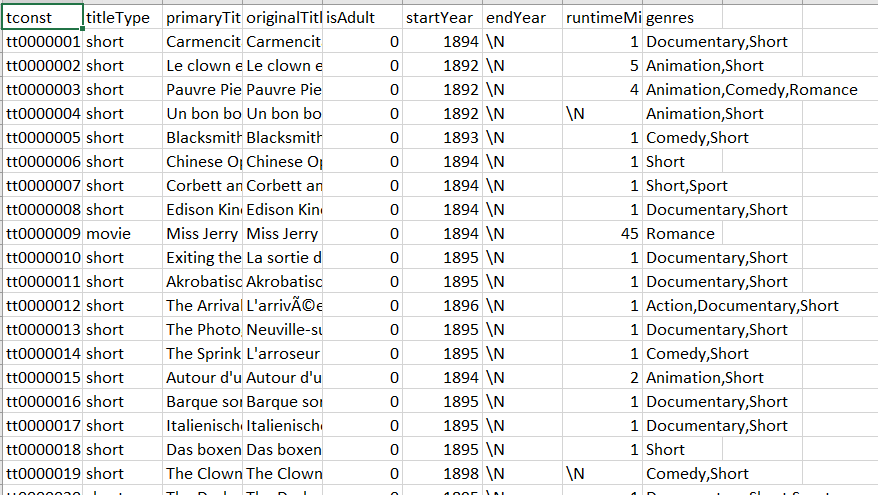
\includegraphics[width = \linewidth]{sample.png}
	\caption{Sample data from table title}
	\label{sample}
\end{figure}
\section{Project Outline}
\subsection{Data Modeling}
In this phase, we understand and explore the data to identify entities, their relations, and constraints. The outcome of this phase will be an  ER diagram that summarizes the observations.
\subsection{Schema Identification}
This phase involves the identification of the schema, and the appropriate constraints and keys required to maintain data integrity and avoid redundancies. Finally, we populate the data in the database.
\subsection{Create Queries}
The next phase in the project will involve identifying possible use-case scenarios of the dataset and building equivalent queries to handle these possible requests. These queries will include searching by title, actor, genre, or other attributes. This phase will be developed in SQL. 
\subsection{User Interface Development}
In this phase, we develop a user-friendly interface for potential customers to interact with the database without having to create their own queries. 
\section{Learning Outcomes}
By the end of the project, we will be able to navigate the domain of big data, identify potential issues in the data, correct and model it efficiently to a relational database management system. 
\end{document}